\subsection{Relational Databases}
The group last year chose to implement the \texttt{WordCount} (see Section \ref{sec:Sprint2And3}) and \texttt{Fuseki} databases using PostgreSQL.
Postgres is a relational database system \cite{knox2020}.


A relational database consists of several layers.
The lowest level is the physical layer which describes how the data are stored physically.
The purpose of the relational model is to abstract over the physical layer of the database.
This abstraction is known as the logical layer and allows database administrators to manage the physical storage without directly manipulating the physical data representation.
The logical layer describes what data are stored and the relationships between the data.
The highest of abstraction is the view layer which describes only part of the database. It exists to simplify the interaction with the system. Many views may exist for the same database.
\cite[Chapter 1.3]{DBSBook}

Compared to storing data on a regular file system, a database system provides many advantages including atomicity of operations, concurrent access to data, and lowered inconsistency and redundancy of data \cite[Chapter 1.2]{DBSBook}.
These advantages can be directly seen in the ACID properties that databases adhere to when performing a transaction (see Section \ref{sec:SQL}) \cite[Chapter~17]{DBSBook}.
\begin{itemize} \label{ACID}
    \item Atomicity: A transaction must either be fully completed or partial side-effects of a failed transaction must be undone.
    \item Consistency: A transaction in isolation must ensure values remain consistent after a transaction has been completed or terminated.
    \item Isolation: Transactions are unaware of other transactions being executed concurrently to avoid confusion.
    \item Durability: Changes caused by a committed transaction persist even in the event of system failures.
\end{itemize}

In the coming sections, we will describe how one can model and describe a relational database design, both mathematically and with a more graphic design.
After doing this, we will examine how operations on these models can be described using SQL (Section~\ref{sec:SQL}) and relational algebra (Section~\ref{sec:relationalAlgebra}).

\subsubsection*{Mathematical description}
Relational database systems can be mathematically described using relations and sets, mapping a unique key to a tuple of information \cite[Chapter~2.3]{DBSBook}.
The values of the tuples contained within the relation can be described by the attributes of the relation and their corresponding domains \cite{KatjaFirstPP}. 
The relations are often described using a \textit{relational schema}, denoting the name and domains of the attributes.

Equation \ref{eq:relational_schema} shows an example of a relation describing books as tuples containing three text fields and a positive integer.
The relation also denotes a super key for the relation. A super key is one or more attributes that can uniquely identify a tuple in a given relation. Attributes describing the super key are underlined.

\begin{equation} \label{eq:relational_schema}
    book(author\_name:text, title: text, number\_of\_pages:\mathbb{Z}^+, \underline{ISBN: text})
\end{equation}
Super keys can be defined as $t_1 \in r,\neq t_2 \in r \implies t_1.K \neq t_2.K$. 

That is, no two tuples $t_1, t_2$ from relation $r$ have same values for all super key attributes $K$. 
If the super key does not contain extraneous attributes, it is said to be \textit{minimal}. \cite[Chapter 2.3]{DBSBook}
We will use the term \textit{primary key} to denote a chosen super key of a relation. 
When describing a database, it is often necessary to specify how various data are connected. 
To do this, one can use \textit{foreign keys} to denote that tuples of $r_1$ is related to a tuple of $r_2$.


One could model the relationship between a book owner and a book using the relational schemas seen in Equation \ref{eq:bookOwnerExample} and \ref{eq:relational_schema}.
There, primary keys from other relations are used to reference unique tuples. The $owns$ relation describes how $book$ and $book\_owner$ are connected. 
\begin{equation}\label{eq:bookOwnerExample}
    \begin{split}
        owns(\underline{owner\_id \rightarrow book\_owner}, \underline{ISBN \rightarrow book}), \\
        book\_owner(name:text,\underline{owner\_id:\mathbb{Z}^+})
    \end{split}
\end{equation}

Instead of describing the data structures of the database in these relations, one can use a different model that represents the logic of the relational schemas.

\subsubsection{Entity relation model}\label{sec:EntityRelationModel}
\begin{figure}
    \centering
    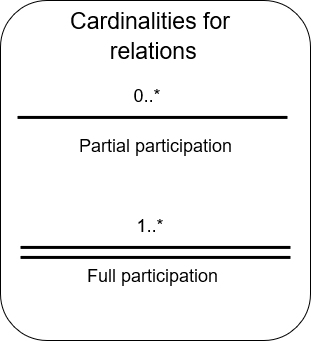
\includegraphics[scale=0.5]{Images/cardinalities.png}
    \caption{Participation ratios for ER relationships}
    \label{fig:ERDiagram_Cardinality}
\end{figure}


Having established the mathematical foundations for how databases function and how to one can model the structure of the data, we will now describe how operations can be performed on the tuples within the relation.

\subsubsection{Relational algebra}\label{sec:relationalAlgebra}
Relational algebra describes a set of unary and binary operations on relations that produce new relations.
These operators form the foundations of data manipulation languages (see Section \ref{sec:SQL}) which can be used to define database operations \cite[Chapter 6.2]{DBSBook}.
We will describe some of the operators of relational algebra, and use them to describe implemented queries later.

\begin{table}[h]
    \centering
    \begin{tabular}{|lll|}
    \hline 
    \multicolumn{1}{|l|}{\textbf{Operator}}          & \multicolumn{1}{l|}{\textbf{Example}}   & \multicolumn{1}{l|}{\textbf{Is unary}}      \\ \hline
    \multicolumn{1}{|l|}{Select}                     & \multicolumn{1}{l|}{$\sigma_{predicate}(R)$}             & \multicolumn{1}{l|}{$\checkmark$}           \\ \hline
    \multicolumn{1}{|l|}{Projection}                 & \multicolumn{1}{l|}{$\pi_{A_1, A2,...,A_n}(R)$}             & \multicolumn{1}{l|}{$\checkmark$}           \\ \hline
    \multicolumn{1}{|l|}{Join}                       & \multicolumn{1}{l|}{$r_1 \Join r_2$}             & \multicolumn{1}{l|}{$\times$}           \\ \hline
    \multicolumn{1}{|l|}{Theta Join}                 & \multicolumn{1}{l|}{$r_1 \Join_\Theta r_2$}             & \multicolumn{1}{l|}{$\times$}           \\ \hline
    \multicolumn{1}{|l|}{Cartesian product}          & \multicolumn{1}{l|}{$r_1\times r_2$}              & \multicolumn{1}{l|}{$\times$}            \\ \hline
    \end{tabular}
    \caption{Table of operators}
    \label{Relational algebra operators}
\end{table}



\subsubsection{SQL}\label{sec:SQL}

Data from a relational database can be queried using relational query languages such as SQL.
Executing a query instructs the database system to perform a set of operations to compute a desired result. Collectively, the resulting set of operations is known as a transaction.
